% !TEX program = xelatex
\documentclass[withoutpreface]{cumcmthesis}

\title{海上油田人员直升机运载计划编排的建模与优化}

\begin{document}

\maketitle

\begin{abstract}
待填充
\keywords{待填充}
\end{abstract}

% ==================== 问题重述 ====================
\section{问题重述}

\subsection{问题背景}

海上油田由多个油气田及配套生产设施构成，生产运行、安全管理、设备维修和后勤保障等环节均需要不同专业人员长期驻守，共同保障油田安全稳定运行。海岗员工通常在设施上连续工作和生活一段时间，到期后集中换班：换班时接班人员出海、离岗人员返回陆地，生产任务和检维修安排的变化还会带来不同海上设施之间的人员穿梭，人员往返主要依靠直升机运输。据此，将人员从陆地机场运往海上设施的运输称为“\textbf{出海}”，从海上设施返回陆地机场的运输称为“\textbf{海返}”，从一座海上设施前往另一座海上设施的运输称为“\textbf{穿梭}”。

\subsection{问题提出}

本题涉及 3 座陆地机场（A01、A02、A03）和 52 座海上设施（F001--F052），其中 8 座设施（F006、F011、F018、F024、F031、F038、F044、F050）设有加油站，位置分布如图~\ref{fig:location} 所示。附件 \texttt{distances.csv} 给出了机场与海上设施两两之间的相对距离（单位：km）。可用机型为 T1、T2、T3 三种，座位数分别为 12、16、19 座，飞行速度分别为 250、220、190 km/h，单位距离油耗分别为 3.4、2.5、2.9 kg/km，油箱容量与最低安全余油量亦各不相同。

\begin{figure}[htbp]
\centering
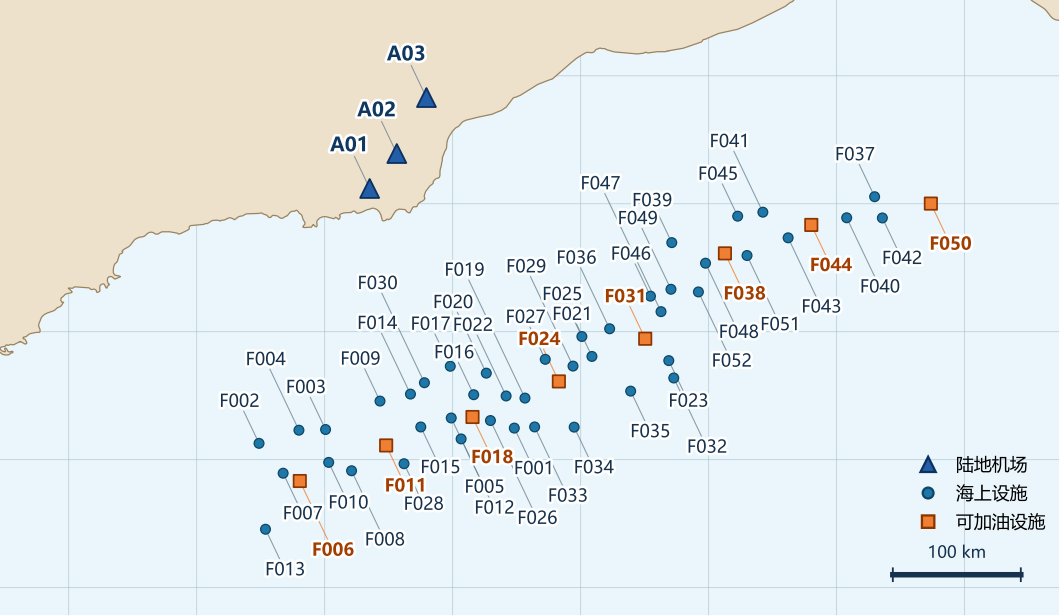
\includegraphics[width=0.72\textwidth]{../figures/问题重述/位置分布.png}
\caption{三座陆地机场与海上设施位置分布}
\label{fig:location}
\end{figure}

一个架次表示一架直升机从机场起飞，连续停靠一座或多座海上设施，在各设施送下或接上人员，最后返回原机场的过程，途中不得在另一座机场中转或结束任务；每个架次最多 5 次海上着陆，人员须由同一个架次运送、不得换乘其他直升机。飞机从机场满油起飞，到达每一地点（含最终返回机场）时剩余燃油不得低于该机型的最低安全余油量；在可加油设施停靠时可选择是否加油（加油时加满），不加油停靠至少 10 分钟、加油停靠至少 20 分钟。本题不考虑机场、海上设施和加油站的并发容量限制。

本题的主要考核目标为\textbf{总飞机使用时间}，即各架次自起飞至返回的时间之和（含各航段飞行与海上停靠）；此外还需考虑\textbf{人员在途时间、座位利用率与总燃油消耗量等}指标。

\textbf{问题一（单向出海运输）}：\texttt{peopleQ1.csv} 给出了 1600 条出海需求。不考虑最早可登机时间、最晚需到达时间和业务性质优先级的约束，假设有足够多的飞机可用于运载，要求在最小化总飞机使用时间的基础上尽可能优化座位利用率、油耗等其他因素，将结果写入 \texttt{q1-assignments.csv} 和 \texttt{q1-routes.csv}，并在论文中给出总飞机使用时间、人员总在途时间、总架次数、总燃油消耗量以及座位利用率。

\textbf{问题二（出海、海返与穿梭联合运输）}：\texttt{peopleQ2.csv} 给出了 4000 条包括出海、海返和穿梭的需求（出海 1600 条、海返 1600 条、穿梭 800 条）。同样不考虑时间窗与优先级约束，假设有足够多的飞机可用，要求在最小化总飞机使用时间的基础上尽可能优化其他因素，将结果写入 \texttt{q2-assignments.csv} 和 \texttt{q2-routes.csv}，并给出上述五项指标。

\textbf{问题三（带时间要求的多日排班）}：\texttt{peopleQ3.csv} 在 \texttt{peopleQ2.csv} 的基础上增加了最早离开起点时刻、最晚送达时刻和业务性质，需求时间在 2026-08-03 至 2026-08-10 之间。需考虑表 3 所列 24 架飞机（按“机场—机型—序号”编号）的数量限制，每架飞机在规划开始时停放在所属机场。机场运营时段内飞机可在 06:00 至 18:00 之间起飞，且不可晚于 20:00 返回机场，不得在海上设施过夜；一架飞机完成一个架次返回原机场后，至少经过 30 分钟机场周转才能再次起飞。临时任务可能为减少运输开销而被取消：先在不考虑临时任务的情况下编排运载计划得到其总飞机使用时间，再在不超过该总飞机使用时间的条件下加入临时人员，尽可能多地满足临时人员运输需求并优化其他因素，将结果写入 \texttt{q3-assignments.csv} 和 \texttt{q3-routes.csv}。

% ==================== 问题分析 ====================
\section{问题分析}

\subsection{问题一的分析}
待填充

\subsection{问题二的分析}
待填充

\subsection{问题三的分析}
待填充

% ==================== 问题假设 ====================
\section{问题假设}
待填充

% ==================== 符号说明 ====================
\section{符号说明}

\begin{table}[htbp]
\centering
\caption{符号说明}
\label{tab:notation}
\begin{tabular}{cll}
\toprule
符号 & 含义 & 单位 \\
\midrule
待填充 & 待填充 & 待填充 \\
待填充 & 待填充 & 待填充 \\
待填充 & 待填充 & 待填充 \\
\bottomrule
\end{tabular}
\end{table}

% ==================== 问题一 ====================
\section{问题一：单向出海运输}
待填充

% ==================== 问题二 ====================
\section{问题二：出海、海返与穿梭联合运输}
待填充

% ==================== 问题三 ====================
\section{问题三：带时间要求的多日排班}
待填充

% ==================== 结果分析与检验 ====================
\section{结果分析与检验}
待填充

% ==================== 模型评价与推广 ====================
\section{模型评价与推广}
待填充

% ==================== 参考文献 ====================
\begin{thebibliography}{99}
% 待填充：使用 BibTeX（gbt7714-2005.bst）或 thebibliography 环境填写参考文献
\end{thebibliography}

% ==================== 附录 ====================
\appendix
\section{附录}
待填充

\end{document}
